\documentclass[11pt]{article}

\usepackage{float}
\usepackage{hyperref}
\usepackage{graphicx}
% formatting
\usepackage{verbatim}
\usepackage{moreverb}
\usepackage{minted}
\usepackage{parskip}
\usepackage{amsmath}
\usepackage[listings]{tcolorbox}
\usepackage{enumerate}
\let\verbatiminput=\verbatimtabinput
\def\verbatimtabsize{4\relax}

\newcommand{\RepoRootPath}{fpga\_labs\_fa19}

\tcbset{
texexp/.style={colframe=black, colback=lightgray!15,
         coltitle=white,
         fonttitle=\small\sffamily\bfseries, fontupper=\small, fontlower=\small},
     example/.style 2 args={texexp,
title={Question \thetcbcounter: #1},label={#2}},
}

\newtcolorbox{texexp}[1]{texexp}
\newtcolorbox[auto counter]{texexptitled}[3][]{%
example={#2}{#3},#1}

\setlength{\topmargin}{-0.5in}
\setlength{\textheight}{9in}
\setlength{\oddsidemargin}{0in}
\setlength{\evensidemargin}{0in}
\setlength{\textwidth}{6.5in}

% Useful macros

\newcommand{\note}[1]{{\bf [ NOTE: #1 ]}}
\newcommand{\fixme}[1]{{\bf [ FIXME: #1 ]}}
\newcommand{\wunits}[2]{\mbox{#1\,#2}}
\newcommand{\um}{\mbox{$\mu$m}}
\newcommand{\xum}[1]{\wunits{#1}{\um}}
\newcommand{\by}[2]{\mbox{#1$\times$#2}}
\newcommand{\byby}[3]{\mbox{#1$\times$#2$\times$#3}}


\newenvironment{tightlist}
{\begin{itemize}
 \setlength{\parsep}{0pt}
 \setlength{\itemsep}{-2pt}}
{\end{itemize}}

\newenvironment{titledtightlist}[1]
{\noindent
 ~~\textbf{#1}
 \begin{itemize}
 \setlength{\parsep}{0pt}
 \setlength{\itemsep}{-2pt}}
{\end{itemize}}

% Change spacing before and after section headers

\makeatletter
\renewcommand{\section}
{\@startsection {section}{1}{0pt}
 {-2ex}
 {1ex}
 {\bfseries\Large}}
\makeatother

\makeatletter
\renewcommand{\subsection}
{\@startsection {subsection}{1}{0pt}
 {-1ex}
 {0.5ex}
 {\bfseries\normalsize}}
\makeatother

% Reduce likelihood of a single line at the top/bottom of page

\clubpenalty=2000
\widowpenalty=2000

% Other commands and parameters

\pagestyle{myheadings}
\setlength{\parindent}{0in}
\setlength{\parskip}{10pt}

% Commands for register format figures.

\newcommand{\instbit}[1]{\mbox{\scriptsize #1}}
\newcommand{\instbitrange}[2]{\instbit{#1} \hfill \instbit{#2}}



\begin{document}

\def\PYZsq{\textquotesingle}
\title{\vspace{-0.4in}\Large \bf EECS 151/251A FPGA Lab 3:\\Tone Generator, Simulation, Connecting Modules, and Memories\vspace{-0.1in}}

\author{Prof. Borivoje Nikolic and Prof. Sophia Shao \\
TAs: Cem Yalcin, Rebekah Zhao, Ryan Kaveh, Vighnesh Iyer \\ Department of Electrical Engineering and Computer Sciences\\
College of Engineering, University of California, Berkeley}
\date{}
\maketitle


\newcommand{\headertext}{EECS 151/251A FPGA Lab 2: Simulation and Sequential Circuits}
\markboth{\headertext}{\headertext}
\thispagestyle{empty}

\section{Before You Start This Lab}

Before you proceed with the contents of this lab, we suggest that you look through these two documents that will help you better understand some Verilog constructs.

\begin{enumerate}
  \item \href{http://inst.eecs.berkeley.edu/~eecs151/fa19/files/verilog/wire_vs_reg.pdf}{wire\_vs\_reg.pdf} - The differences between wire and reg nets and when to use each of them.
  \item \href{http://inst.eecs.berkeley.edu/~eecs151/fa19/files/verilog/always_at_blocks.pdf}{always\_at\_blocks.pdf} - Understanding the differences between the two types of always @ blocks and what they synthesize to.
\end{enumerate}

\section{Designing a Tone Generator}
Let's create a tone generator/buzzer on the FPGA.

\subsection{Clock Sources}
Look at the \href{https://reference.digilentinc.com/reference/programmable-logic/pynq-z1/reference-manual}{Pynq Reference Manual}.
Read Section 11 about the clock sources available on the Pynq.
We are using the 125 MHz clock from the Ethernet PHY IC on the Pynq board connected to pin H12 of the FPGA chip.

Look at the \texttt{src/z1top.v} top-level module and its \verb|CLK_125MHZ_FPGA| input.
\begin{minted}{verilog}
module z1top (
    input CLK_125MHZ_FPGA,
    ...
);
\end{minted}
Next take a look at the constraints in \texttt{src/PYNQ-Z1\_C.xdc} and notice how the LOC for the clock net is set to H16, just as specified in the Pynq-Z1 Reference Manual.
\begin{minted}{tcl}
set_property -dict { PACKAGE_PIN H16 IOSTANDARD LVCMOS33 } \
  [get_ports { CLK_125MHZ_FPGA }];
\end{minted}
This is how we map top-level signals in Verilog to the physical FPGA pins they are connected to.
We can access the clock signal from our Verilog top-level module and can propagate this clock signal to any submodules that may need it.

\subsection{Audio Out}
Look at Section 14 of the \href{https://reference.digilentinc.com/reference/programmable-logic/pynq-z1/reference-manual}{Pynq Reference Manual} which describes the mono audio out feature on the Pynq board.

The FPGA pin R18 is connected to the \verb|AUD_PWM| net.
The FPGA can drive this net with a PWM signal which goes through a low-pass filter and is driven into the audio jack on the Pynq board.

There's also an \verb|AUD_SD| net connected to FPGA pin T17, which turns off the opamps in the low-pass filter.
Setting \verb|AUD_SD| to 1 enables the audio output.

Find these signals in the \texttt{src/PYNQ-Z1\_C.xdc} file, and note how they appear in the \texttt{src/z1top.v} port list.

\subsection{Generating a Square Wave}
Let's play a 220 Hz square wave out of the Mono Audio Out port on the Pynq.
The square wave should have a 50\% duty cycle, so for half of the period of one wave the signal should be high and for the other half, the signal should be low.
We have a 125 MHz clock we can use to time our circuit.

Find the following:
\begin{texexptitled}{Square Wave Calculations}{}
\begin{enumerate}[a)]
\item The period of our clock signal (frequency = 125 MHz)?
\item The period of a 220 Hz square wave?
\item How many clock cycles fit in one period of the square wave?
\end{enumerate}
\end{texexptitled}

Open \verb|src/tone_generator.v| and design a circuit to output a 220Hz square wave on the \verb|square_wave_out| output.
Ignore the \verb|tone_switch_period|, \verb|output_enable|, and \verb|volume| inputs for now.

\section{Simulating the Tone Generator}
Let's run some simulations on the \verb|tone_generator| in software to check it works before putting it on the FPGA.
To do this, we will need to use a Verilog testbench.
A Verilog testbench is designed to test a Verilog module by supplying it with the inputs it needs (stimulus signals) and testing whether the outputs of the module match what we expect.

\subsection{Overview of Testbench Skeleton}
Check the provided testbench skeleton in \verb|sim/tone_generator_testbench.v|.
Let's go through what every line of this testbench does.

\begin{minted}{verilog}
`timescale 1ns/1ns
\end{minted}

The timescale declaration needs to be at the top of every testbench file.
\begin{minted}{verilog}
`timescale (simulation step time)/(simulation resolution)
\end{minted}

The first argument to the timescale declaration is the simulation step time.
It defines the granularity of discrete time units in which the simulation advances.
In this case, we have defined the simulation step time to be one nanosecond, so we can advance the simulation time by as little as 1ns at a time.

The second argument to the timescale declaration is the simulation resolution.
In our example it is also 1ns.
The resolution allows the simulator to model transient behavior of your circuit in between simulation time steps.
For this lab, we aren't modeling any gate delays, so the resolution can safely equal the step time.

\begin{minted}{verilog}
`define SECOND 1000000000
`define MS 1000000
// The SAMPLE_PERIOD corresponds to a 44.1 kHz sampling rate
`define SAMPLE_PERIOD 22675.7
\end{minted}

These are some macros defined for our testbench.
They are constant values you can use when writing your testbench to simplify your code and make it obvious what certain numbers mean.
For example, \verb|SECOND| is defined as the number of nanoseconds in one second.
The \verb|SAMPLE_PERIOD| is the sampling period used to sample the square wave output of the \verb|tone_generator| at a standard 44.1 kHz sample rate.

\begin{minted}[tabsize=4]{verilog}
module tone_generator_testbench();
  // Testbench code goes here
endmodule
\end{minted}

\verb|tone_generator_testbench| is a testbench module.
It is not intended to be placed on an FPGA, but rather it is to be run by a circuit simulator.
All your testbench code goes in this module.
We will instantiate our DUT (device under test) in this module.

\begin{minted}{verilog}
reg clock;
reg output_enable;
reg volume = 0;
reg [23:0] tone_to_play;
wire sq_wave;
\end{minted}

Here are the inputs and outputs of our \verb|tone_generator|.
Notice that the inputs to the \verb|tone_generator| are declared as \verb|reg| type nets and the outputs are declared as \verb|wire| type nets.
This is because we will be driving the inputs in our testbench inside an \verb|initial| block and we will be reading the output.
Note we can set the initial value of \verb|reg| nets in the testbench to drive a particular value into the DUT at time 0 (e.g. \verb|volume|).

\begin{minted}{verilog}
initial clock = 0;
always #(4) clock <= ~clock;
\end{minted}

This is the clock generation code.
The clock signal needs to be generated in our testbench so it can be fed to the DUT.
The initial statement sets the value of the clock net to 0 at the very start of the simulation.
The next line toggles the clock signal every 4ns, i.e. half period of 125 MHz clock.

\begin{minted}[tabsize=4]{verilog}
tone_generator audio_controller (
    .clk(clock),
    .output_enable(output_enable),
    .tone_switch_period(tone_to_play),
    .volume(volume),
    .square_wave_out(sq_wave)
);
\end{minted}

Now we instantiate the DUT and connect its ports to the nets we have declared in our testbench.

\begin{minted}[tabsize=4]{verilog}
initial begin
    tone_to_play = 24'd0;
    output_enable = 1'b0;
    #(10 * `MS);
    output_enable = 1'b1;

    tone_to_play = 24'd37500;
    #(200 * `MS);
    ...
    $finish();
end
\end{minted}

This is the body of our testbench.
The \verb|initial begin ... end| block is the `main()' function for our testbench, and where the simulation begins execution.
In the \verb|initial| block we drive the DUT inputs using blocking (\verb|=|) assignments.

We can also order the simulator to advance simulation time using delay statements.
A delay statement takes the form \verb|#(delay in time steps);|.
For instance the statement \verb|#(100);| would run the simulation for 100ns.

In this case, we set \verb|output_enable| to 0 at the start of the simulation, let the simulation run for 10ms, then set \verb|output_enable| to 1.
Then \verb|tone_to_play| is changed several times, and the \verb|tone_generator| is given some time to produce the various tones.

The final statement is a system function: the \verb|$finish()| function tells the simulator to halt the simulation.

\begin{minted}[tabsize=4]{verilog}
integer file;
initial begin
  file = $fopen("output.txt", "w");
  forever begin
    $fwrite(file, "%h\n", sq_wave);
    #(`SAMPLE_PERIOD);
  end
end
\end{minted}

This piece of code is written in a separate \verb|initial begin ... end| block.
The simulator treats both \verb|initial| blocks as separate threads that both start execution at the beginning of the simulation and run in parallel.

This block of code uses two system functions \verb|$fopen()| and \verb|$fwrite()|, that allow us to write to a file.
The \verb|forever begin| construct tells the simulator to run the chunk of code inside it continuously until the simulation ends.

In the \verb|forever begin| block, we sample the \verb|square_wave_out| output of the \verb|tone_generator| and save it in \verb|output.txt|.
We sample this value every \verb|`SAMPLE_PERIOD| nanoseconds which corresponds to a 44.1 kHz sampling rate.
The \verb|tone_generator|'s output is stored as 1s and 0s in \verb|output.txt| that can be converted to an audio file to hear how your circuit will sound when deployed on the FPGA.

\subsection{Running the Simulation}
There are 3 RTL simulators we can use:
\begin{itemize}
  \item \textbf{VCS} - proprietary, only available on lab machines, fastest
  \item \textbf{XSIM} - free, bundled with Vivado, somewhat slower
  \item \textbf{Icarus Verilog} - open source, runs on Windows/OSX/Linux, somewhat slower
\end{itemize}
They all take in Verilog RTL and a Verilog testbench module and output:
\begin{itemize}
  \item A waveform file (.vpd, .vcd) that plots each signal in the testbench and DUT across time
  \item A text dump containing anything that was printed during the testbench execution
\end{itemize}

\subsubsection{VCS}
If you're using the lab machines, you should use VCS:
\begin{minted}{bash}
  make sim/tone_generator_testbench.vpd
\end{minted}
This will generate a waveform file \verb|sim/tone_generator_testbench.vpd| which you can view using \verb|dve|.
Login to the lab machines physically or use X2go and run:
\begin{minted}{bash}
  dve sim/tone_generator_testbench.vpd &
\end{minted}

\textbf{TODO} insert a screenshot of dve and how to use it
\begin{enumerate}
	\item \textbf{Module Window} - List of the modules involved in the testbench. You can select one of these to have its signals show up in the object window.
	\item \textbf{Object Window} - List of all the wires and regs in the selected module. You can add signals to the waveform view by selecting them, right-clicking, and doing \verb|Add Wave|.
	\item \textbf{Waveform Viewer} - The signals that you add from the object window show up here. You can navigate the waves by searching for specific values or going forward or backward one transition at a time. The x-axis represents time.
\end{enumerate}

Here are a few useful shortcuts:

\begin{itemize}
	\item \textbf{Click on waveform}: Sets cursor position
	\item \textbf{O}: Zoom out of waveform
	\item \textbf{I}: Zoom into waveform
	\item \textbf{F}: Fit entire waveform into viewer (zoom full)
	\item \textbf{C}: Zoom in on cursor position
	\item \textbf{Middle Click + Drag Left/Right}: Zoom in on waveform section
	\item \textbf{Middle Click + Drag to Top Right}: Zoom out from current waveform section
\end{itemize}

\subsubsection{XSIM}
Vivado has an integrated simulator, \textbf{xsim}, that can run your Verilog testbench.
You can run XSIM on your laptop.

\textbf{TODO} open waveforms with dve or gtkwave

\textbf{TODO} add vivado bin to PATH, how to run tests, how to view waves with gtkwave

\subsubsection{iverilog}
\textbf{TODO} how to install on linux/osx/windows, how to run tests

Let's go over the basics of ModelSim. The boxed screens are:

\subsection{Analyzing the Simulation}
You should be able to see the clock oscillate at the frequency specified in the testbench.
You should also see the \verb|output_enable| signal start at 0 and then become 1 after 10 ms.
However, you may see that the \verb|sq_wave| signal is just a red line. What's going on?

\subsubsection{Fixing the Undefined clock\_counter}
Blue lines (written as `Z' in Verilog) in a waveform viewer indicate high-impedance (unconnected) signals.
We won't be using high-impedance signals in our designs, so blue lines or `Z' indicate something in our testbench or DUT isn't wired up properly.

If you have a red line for your \verb|clock_counter| at the start of your simulation, it may be because the initial value sitting inside the \verb|clock_counter| register is unknown. It could be anything! Since we don't have an explicit reset signal for our circuit to bring the \verb|clock_counter| to a defined value, it may be unknown for the entire simulation.

Let's fix this. In the future we will use a reset signal, but for now let's use a simpler technique. In \verb|lab2/src/tone_generator.v| modify this line as such:

\begin{minted}{verilog}
// Original code:
reg [x:0] clock_counter;

// Change to:
reg [x:0] clock_counter = 0;
\end{minted}

This tells the simulator that the initial value for this register should be 0. For this lab, when you add new registers in your \verb|tone_generator| or any other design module, you should instantiate them to their initial value in the same way. \textbf{Do not set an initial value for a 'wire' type net; it will cause issues with synthesis, and may cause X's in simulation.}

Now run the simulation again.

\subsubsection{Helpful Tip: Reloading ModelSim .wlf}

When you re-run your simulation and you want to plot the newly generated signals in ModelSim, you don't need to close and reopen ModelSim. Instead click on the 'Reload' button on the top toolbar which is to the right of the 'Save' button.

\subsubsection{Listen to Your Square Wave Output}

Take a look at the file written by the testbench located at \verb|lab3/sim/build/output.txt|. It should be a sequence of 1s and 0s that represent the output of your \verb|tone_generator| sampled at 44.1 kHz. Use a Python script that can take this file and generate a \verb|.wav| file that you can listen to.

Go to the \verb|lab3/| directory and run the command:

\verb|python scripts/audio_from_sim.py sim/build/output.txt|

This will generate a file called \verb|output.wav|. Run this command to play it:

\verb|play output.wav|

If \verb|play| doesn't work, try running \verb|aplay output.wav|.

You should hear 5 tones, played rapidly one after the other that have descending frequencies.

\subsubsection{Playing with the Testbench} \label{checkoff:0}

Play around with the testbench by altering the clock frequency, changing when you turn on \verb|output_enable| and verifying that you get the audio you expect. For checkoff be able to answer the following questions and demonstrate understanding of simulation:

\begin{enumerate}
	\item If you increase the clock frequency from 125 Mhz, would you expect the tones generated by your \verb|tone_generator| to be of a higher or lower frequency than was generated with the 125 MHz clock? Why? Show audio evidence of this using simulation.
	\item Prove that the \verb|output_enable| input of your \verb|tone_generator| actually works in simulation.
	\item Create a testbench that plays some simple melody that you define and have its audio output file ready for checkoff.
\end{enumerate}

\subsection{Vivado's Integrated Simulator}

Inside a Vivado project, expand the \emph{Simulation Sources} category in your \emph{Project Hierarchy} window (that's the one with all your files). At any given time only one Verilog module can be the simulation ``Top'', just as there can only be one synthesis ``Top'' for implementation. If it isn't already, right-click \verb|tone_generator_testbench| and select \emph{Set As Top}. Then in the \emph{Flow Navigator} window, click \emph{Run Simulation} in the \emph{Simulation} category. You will get a context menu: select \emph{Run Behavioural Simulation}.

Then you will be presented with the Vivado Simulation window:

\begin{figure}[H]
	\centerline{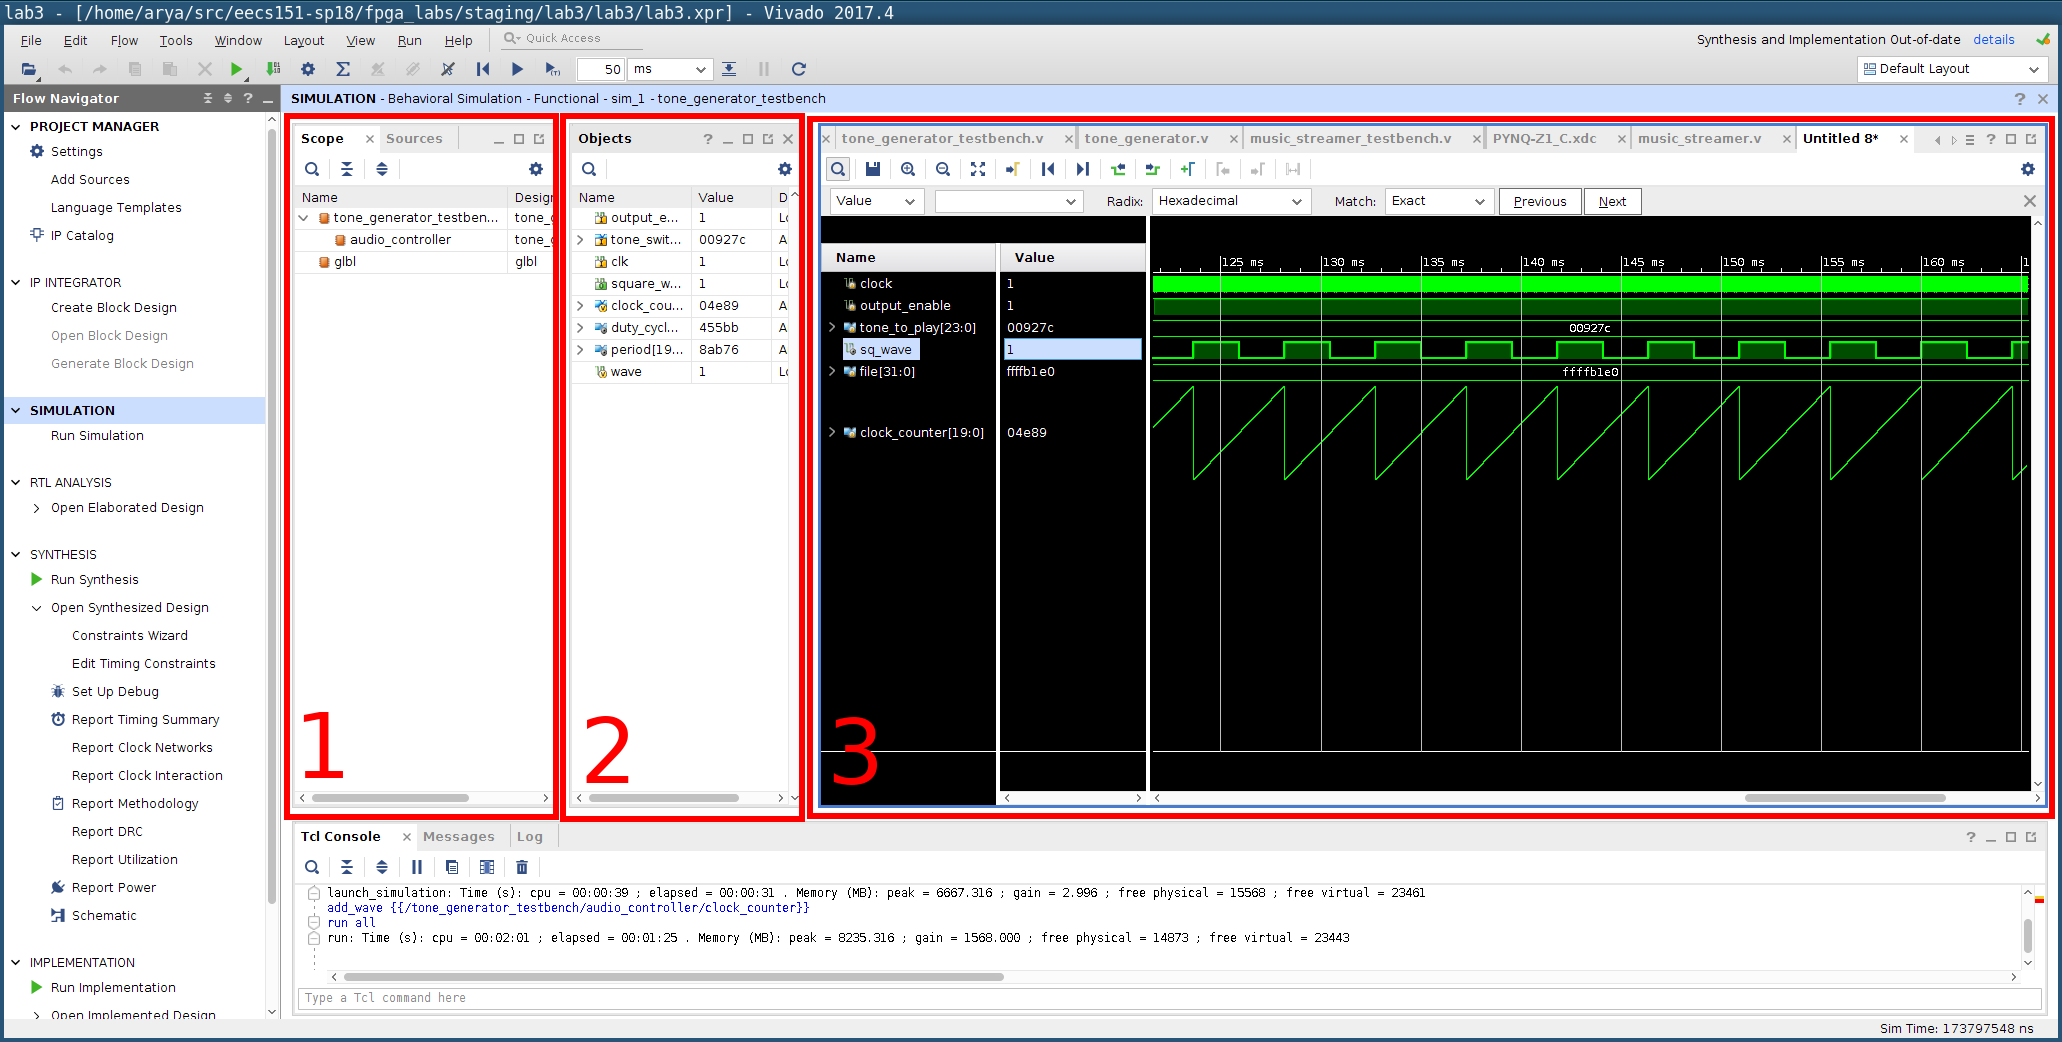
\includegraphics[width=\textwidth]{figs/vivado_xsim.png}}
\end{figure}

This should be familiar to you: it looks and behaves like the ModelSim GUI you saw earlier.

\begin{enumerate}
  \item is the \textbf{Scope Window}, which is like ModelSim's \textbf{Module Window}, and lets you select from among simulated modules;
  \item is an \textbf{Object Window} just like ModelSim's, allowing you to select waveforms to view; and
  \item is the \textbf{Waveform Viewer}.
\end{enumerate}

Play around with it; does your intuition from ModelSim carry over?

Although the Vivado simulator can be controlled with a Tcl script like ModelSim, there is a GUI way to modify settings too. Click \emph{Tools} menu $\rightarrow$ \emph{Settings} to bring up the \emph{Project Settings} dialog. Select the \emph{Simulation} category in the left pane. (Notice that you can change the default simulator here from Vivado to, say, ModelSim.) The options defined in various tabs in the right hand pane allow you to select various simulation parameters, including initial duration.

A final note: when the \emph{Simulation} window is open in Vivado, you can use the \emph{Tcl Console} to execute simulation commands. (The \emph{Tcl Console} appears just below boxes (1) - (3) in the figure above.) A lot of the commands you can use here will work like they do for ModelSim. The full list of commands is available in the \href{https://www.xilinx.com/support/documentation/sw_manuals/xilinx2016_1/ug937-vivado-design-suite-simulation-tutorial.pdf}{user manual from Xilinx}.

\subsubsection{Where does Vivado put output.txt?}

The Vivado simulator will also have produced an \verb|output.txt| file with waveform samples. But where? In your project root directory, use \verb|find| to \emph{find} out:

\begin{verbatim}
lab3 $ find . -name "output.txt"
./lab3/lab3.sim/sim_1/behav/xsim/output.txt
\end{verbatim}

\subsection{Resetting Simulations}

Running simulations, both for ModelSim and in Vivado, generates a lot of signal data for the waveforms viewers. You often don't need to keep this intermediary data (which is easily several gigabytes in this lab alone), and you may be running out of quota on the machine you're using. In order to clear intermediate state and reset the simulation, perform the following steps.

\begin{enumerate}
  \item For \textbf{ModelSim}, navigate to the \verb|sim| directory in which you executed \verb|make CASES=|, e.g. \textbf{\RepoRootPath/lab3/sim}. There, execute \verb|make clean|.
  \item For \textbf{Vivado}, open the \emph{Tcl Console}. It's usually available toward the bottom-left of the application window, but can also be opened from the menus. In the Tcl Console, execute \verb|reset_simulation|.
\end{enumerate}

\section{Top-Level Wiring and Tone Generator on the FPGA}

Then open \verb|src/z1top.v| and instantiate the \verb|tone_generator|.
Connect \verb|square_wave_out| to \verb|aud_pwm|.
Set \verb|aud_sd| to 1, to enable the audio output.

Build a bitstream by running \texttt{make impl} in \texttt{\RepoRootPath/lab3}.
Check for any warnings or errors in \texttt{build/synth/latest/synth.log} and try to fix them.
Ask a TA if you need help here.

Program the FPGA by running \texttt{make program}.
Plug in headphones and make sure you hear a buzzing noise at 220Hz; compare the tone with a \href{https://www.szynalski.com/tone-generator/}{reference generator}.
To stop the buzzing, you can press the \verb|SRST| button on the top-right of the Pynq.

%Some starter code is included in this file. Begin by sizing your \verb|clock_counter| register to the number of bits it would take to store the clock cycles per square wave period. Design the logic such that a 220 Hz square wave comes out of the \verb|square_wave_out| output. Instantiate the \verb|tone_generator| inside \verb|z1top.v| and connect it to the Audio Out pin we defined previously. Make sure that you enable the Audio Out with the \verb|aid_sd| signal as well.

%Build your design. Check for any warnings or errors and try to fix them. Ask a TA if you need help here. When everything looks good, program the board. If everything works, you should be able to plug your audio-out signal into a speaker in the lab (or your own earphones) to hear a buzzing noise at 220 Hz. To stop the buzzing, just turn your FPGA off.

\section{Enhancements}
\subsection{Switching the Wave On and Off}
Now you have a tone, but it can't be toggled on and off without pulling the power to the FPGA board. Let's use the \verb|output_enable| input of the \verb|tone_generator| module to gate the square wave output. When \verb|output_enable| is 0, you should pass 0 to the \verb|square_wave_out| output, but when \verb|output_enable| is 1, you should pass your square wave to \verb|square_wave_out|.

Wire up the \verb|output_enable| signal to the first slide switch (\verb|SWITCHES[0]|) in \verb|z1top|.

Run your design flow. Check for any warnings or errors and try to fix them. Ask a TA if you need help here. When everything looks good, program the board through the hardware manager. You should now hear a buzzing noise at 220Hz that can be turned on or off by toggling the first slide switch.

You should verify that the tone is indeed 220 Hz by comparing it to a reference tone here: \url{http://onlinetonegenerator.com/}.

\subsection{Volume Adjustment}

\subsection{Design a Configurable Frequency tone\_generator}

Let's extend our \verb|tone_generator| so that it can play different notes. You may start by adding a 24-bit input to the \verb|tone_generator| called \verb|tone_switch_period|. Note you will also have to modify your \verb|clock_counter| to be 24 bits wide.

The \verb|tone_switch_period| describes how often the square wave output switches from high to low or low to high. For example a \verb|tone_switch_period| of 284091 (0 d.p.) tells us to invert the square wave output every 142045 clock cycles, which for a 125 Mhz clock translates to a $\sim 440$ Hz square wave. Here is the derivation:

\begin{eqnarray}
  \frac{125 \times 10^6 \text{ cycles}}{1 \text{ second}} \div \frac{440 \text{ periods}}{1 \text{ second}} = \frac{ 284091 \text{ cycles}}{1 \text{ period}} \nonumber \\
  284091 \text{ cycles/period} \rightarrow 142045 \text{ cycles/half-period} \nonumber
\end{eqnarray}

You may have to modify the architecture of your \verb|tone_generator| to accommodate this new input signal. You should reset the internal \verb|clock_counter| every \verb|tone_switch_period| cycles and should also invert the square wave output. Remember to initialize any new registers declared in your \verb|tone_generator| to their desired initial value to prevent unknowns during simulation.

You should also handle the case when \verb|tone_switch_period| is 0.  In this case disable the tone output.

\subsubsection{Try the Configurable Frequency tone\_generator on the FPGA}
Modify the top-level Verilog module \verb|z1top.v| to include the new input to the \verb|tone_generator|. You should tie the \verb|tone_switch_period| to \verb|SWITCHES[0]| and \verb|BUTTONS[3:0]|, left-shifted by 9 bits (effectively a multiplication by 512). This will allow you to control the \verb|tone_switch_period| from 512 to 15872. Leave \verb|SWITCHES[1]| to control \verb|output_enable| initially; later, you can use it as an extra bit's worth of input. Here is a code snippet (incomplete):

\begin{minted}[tabsize=4]{verilog}
    tone_generator audio_controller (
        .output_enable(SWITCHES[1]),
        .tone_switch_period({18'd0, SWITCHES[0], BUTTONS[3:0]} << 9),
    );
\end{minted}

What other way(s) do you have to digitally mute your output signal?

Is the width of the bus assigned to \verb|tone_switch_period| correct? Does it matter?

Run the usual synthesis, implementation and programming flow to put your new \verb|tone_generator| on the FPGA. Verify that toggling the switches and buttons changes the frequency of your \verb|tone_generator|.



\section{Introduction to Inferred Asynchronous ROMs}
An asynchronous memory is a memory block that isn't governed by a clock. In this lab, we will use a Python script to generate a ROM block in Verilog.

A ROM is a read-only memory. This data can be accessed by supplying an address to the ROM; after some time, the ROM will output the data stored at that address. A memory block in general can contain as many addresses in which to store data as you desire. Every address should contain the same amount of data (bits). The number of addresses is called the \textbf{depth} of the memory, while the number of bits stored per address is called the \textbf{width} of the memory.

The synthesizer takes the Verilog you write and converts it into a low-level netlist of the structures are actually used on the FPGA. Our Verilog \textbf{describes} the functionality of some digital circuit and the synthesizer \textbf{infers} what primitives implement the functional description. In this section, we will examine the Verilog that allows the synthesizer to infer a ROM. This is a minimal example of a ROM in Verilog: (depth of 8 entries/addresses, width of 12 bits)

\begin{minted}[tabsize=2]{verilog}
module rom (input [2:0] address, output reg [11:0] data);
	always @(*) begin
		case(address)
			3'd0: data = 12'h000;
			3'd1: data = 12'hFFF;
			3'd2: data = 12'hACD;
			3'd3: data = 12'h122;
			3'd4: data = 12'h347;
			3'd5: data = 12'h93A;
			3'd6: data = 12'h0AF;
			3'd7: data = 12'hC2B;
		endcase
	end
endmodule
\end{minted}

To power our \verb|tone_generator|, we will be using a ROM that is X entries/addresses deep and 24 bits wide. The ROM will contain tones that the \verb|tone_generator| will play. You can choose the depth of your ROM based on the length of the sequence of tones you want to play.

We've provided you with a few scripts that can generate a ROM from either a file with it's contents or even from sheet music. Run these commands from \verb|lab3/|.

\begin{minted}{bash}
python scripts/musicxml_parser.py musicxml/Twinkle_Twinkle_Little_Star.mxl music.txt
python scripts/rom_generator.py music.txt ./lab3.srcs/sources_1/new/rom.v 1024 24
\end{minted}

The first script will parse a MusicXML file and turn it into a list of \verb|tone_switch_periods| for each of the notes for a piece of sheet music. The second script will take that list and turn it into a ROM that's 1024 entries deep with a width of 24 bits.

Take a look at \verb|music.txt| and \verb|src/rom.v|. You can download your own music in MusicXML format from here (\url{https://musescore.org/}) and run it through the same parser; it should ideally only have one part to work properly. You can also directly edit the \verb|music.txt| file to customize the contents of the ROM as you wish.

\section{Design of the music\_streamer}
Open up the \verb|music_streamer.v| file. You will need to modify this module to contain an instance of the ROM you created earlier and logic to address the ROM sequentially to play notes. The \verb|music_streamer| will play each note in the ROM for a predefined amount of time by sending it to the \verb|tone_generator|.

We will play each note for 1/25th of a second. Calculate what that is in terms of 125Mhz clock cycles.

Now let's begin the design of the \verb|music_streamer| itself. Instantiate your ROM in the \verb|music_streamer| and connect the ROM's \verb|address| and \verb|data| ports to wire or reg nets that you create in your module.  The \verb|last_address| port outputs the last address in the ROM (depth).

Next, write the RTL that will increment the address supplied to the ROM every \textbf{1/25th of a second}. The data coming out of the ROM should be fed to the \verb|tone| output. The ROM's address input should go from 0 to the depth of the ROM and should then loop around back to 0. You don't have a reset signal, so define the initial state of any registers in your design for simulation purposes. Also hook up the \verb|rom_address| output to the ROM address currently being accessed.

Now that you have implemented \verb|music_streamer|, create an instance of it in the module \verb|z1top.v|. Use the instance name \verb|streamer| to match the expected name in the \verb|.do| file. Instantiate a \verb|tone_generator| and wire \verb|SWITCHES[1]| to \verb|output_enable|, \verb|CLK_125MHZ_FPGA| to \verb|clk|, and \verb|aud_pwm| to \verb|square_wave_out|.  Assign \verb|aud_sd| to 1.  Connect the \verb|tone| output of the \verb|music_streamer| to the \verb|tone_switch_period| input of the \verb|tone_generator|. Connect the \verb|music_streamer|'s \verb|clk| input to the global clock signal. Finally, connect  its \verb|rom_address| output to the \verb|LEDS|s by routing the top 6 bits of address.

\section{Simulating the music\_streamer}
To simulate your \verb|music_streamer| open up the \verb|lab3/src/music_streamer_testbench.v|. In contrast to the \verb|tone_generator_testbench| where the \verb|tone_generator| was instantiated in isolation, in this testbench we are instantiating our entire top-level design, \verb|z1top|. This testbench is referred to as a system-level testbench, which tests our entire design using top-level I/O, in contrast to the \verb|tone_generator_testbench| which is a block-level testbench. This is similar to the difference between unit and integration tests in software development.

You can see that this testbench just runs a simulation for 2 seconds and then exits. You might have to modify the \verb|music_streamer_testbench.do| file to match the name of your module instances in \verb|z1top.v|.

To execute the testbench, run \verb|make CASES=tests/music_streamer_testbench.do| in \verb|lab3/sim|. This may take several minutes to complete. You may have to run \verb|make clean| before running \verb|make| if ModelSim has cached build artifacts.

Inspect your waveform to make sure you get what you expect. Verify that there are no undefined signals (red lines, x) Then run the Python script to generate a \verb|.wav| file of your simulation results and listen to your \verb|music_streamer|. It should sound like the first few seconds of the song that was loaded on the ROM.

\section{Verify your Code Works For Rest Notes}
In simulation, you can often catch bugs that would be difficult or impossible to catch by running your circuit on the FPGA. You should verify that if your ROM contains an entry that is zero (i.e. generate a 0Hz wave), that the \verb|tone_generator| holds the \verb|square_wave_out| output at either 1 or 0 with no oscillation. Verify this in simulation, and prove the correct functionality during checkoff.

\section{Try it on the FPGA!}
Now try your \verb|music_streamer| on the FPGA. You should expect the output to be the same as in simulation. The \verb|SWITCHES[1]| switch should still work to disable the output of the \verb|tone_generator|. Show your final results, simulation, and the working design on the FPGA to the TA for checkoff.

%\section{Optional: Adding Tempo Variations and Pausing to the music\_streamer}
%In the next lab, we will be making our \verb|music_streamer| more full-featured. If you have time now, you can implement some of these features.

%Connect a \verb|BUTTONS| switch to a new \verb|pause| input of the \verb|music_streamer|. When this switch is turned on, your module should pause the music at the current note and should cut the output to the audio out. When the switch is turned off, your module should resume playback.

%Connect a pair of \verb|BUTTONS| switches to a new \verb|tempo| input of the \verb|music_streamer|. When these switches are toggled, your \verb|music_streamer| should play the notes faster or slower. Basically, you can define four different tempos that hold each note for a different amount of time. We choose a standard 1/25th of a second for this lab, but you can vary it from 1/75, 1/50, 1/30, 1/15 to change the tempo of your music playback on the fly.

\section{Saving your Work Using Git}
At the beginning of this lab, you were asked to copy part of your solution lab 2 into this project.  As we continue onto new labs and eventually onto the project, you will be asked to build off of your solution to previous labs.  Given that your lab solutions will be important later in the term, we want to make sure you have a safe place to store your solutions.  To do that, we have provided you with a private git repository on GitHub.

As was mentioned in lab 1, git is a revision control system that can keep track of files in your lab assignments and project.  You have already been using git to get each week's lab assignments.  Starting with this lab, you will also be using git to keep track of your solutions to the lab assignments.

Now let's get your solution committed into the git repository!

\subsection{Adding New Files}
First, git does not automatically track new files that you create.  These files can be added to git using the \verb|git add| command.  If you created any new files during this lab that you want to save, run the following command (replacing \verb|<path to file>| with the path to the file you wish to add):
\begin{minted}[tabsize=2]{bash}
git add <path to file>
\end{minted}

\subsection{Checking Git Status}
We can check to see what git believes the state of the repository is.  Run the following command in the lab3 directory:
\begin{minted}[tabsize=2]{bash}
git status
\end{minted}
You should see a list of many files that you have modified over the course of labs 1, 2, and 3.  This command also shows files that git is not tracking, which are listed under the ``Untracked files'' section.  Check to make sure that files you want to save are not listed in the ``Untracked files'' section.  If they are, add them using \verb|git add|.

\subsection{Committing Your Solution}
We now need to commit your changes to the repository.  Committing a file saves any changes made to the file since the last commit into the repository.  There are several methods to do this:
\begin{itemize}
\item You can use the command \verb|git commit <file/directory list>| to commit files that are in the list specified by \verb|<file/directory list>|.  You should replace \verb|<file/directory list>| with the list of files and/or directories you want to commit.  Use spaces between the different files/directories in the list.
\item You can use the command \verb|git commit -a| to commit every file that has been changed and added with \verb|git add|.
\item You can use the \verb|git add| command to ``stage'' files for commit.  Run \verb|git add| for each file you would like to commit.  Then run \verb|git commit| to commit the staged files.
\end{itemize}

Each of these command will bring up a text editor (probably vim) with a summary of the the actions git is about to take.  It will ask you to type a commit message at the top of the document, save it, and quit the text editor.  If you are comfortable with vim, feel free to enter your commit message, save the file, and exit.  Otherwise, enter \verb|:q!| and press return.  This will exit vim without saving.  Git will give you a message saying that the commit was aborted because of an empty commit message.  You can enter a commit message from the command line by adding the flag \verb|-m "commit message"| to any of the above commands.  You should replace ``commit message'' with some text explaining what you are committing.

\subsection{Setting Up Your Private GitHub Repository - Do this Once Per Clone}
In this class you will interacting with 2 GitHub repositories :
\begin{itemize}
\item a public repository maintained by the lab staff which contains the skeleton code for each lab
\item a private repository where you will store your solutions to the lab
\end{itemize}

Earlier in lab 1, you cloned the public repository maintained by the lab staff.  This repository allows you to pull new updates that the lab staff post.  Your private repository can be viewed via a web browser at \verb|https://github.com/EECS150/sp19-eecs151-####| where \verb|###| is the three characters in your eecs151 instructional account.  Make sure you can access the web page for your repository.  Because it is private, you will need to be signed into GitHub to see it.  You may also need to accept an invitation sent to the e-mail address you registered with GitHub.

Currently, git on your computer is only aware of the public repository.  We need to execute some commands to tell it about your new private repository.

In the \verb|fpga_labs_sp19| directory, run the following commands, replacing \verb|###| with the 3 characters in your eecs151 instructional account:
\begin{minted}[tabsize=2]{bash}
git remote rename origin staff
git remote add origin git@github.com:EECS150/sp19-eecs151-###.git
\end{minted}

You will need to repeat these steps each time you clone the \verb|fpga_labs_sp19| repository.

\subsection{Pushing Updates to your Private GitHub Repository}
Now that you have your files committed into the git repo, you need to push your updates to the GitHub server.  To do this, run the following command:
\begin{minted}[tabsize=2]{bash}
git push origin master
\end{minted}

If you gave a password with your ssh key, enter it when prompted.  You should then see messages indicating that git is pushing your updates to your private repository!

Go to \verb|https://github.com/EECS150/sp19-eecs151-###| and check that your files made it.

\subsection{Pulling from GitHub}
From this point forward, you will use this command to get new lab content from the course staff:
\begin{minted}[tabsize=2]{bash}
git pull staff master
\end{minted}

If you are on a different computer (ex. a home computer) and want to pull any of the solutions you committed and pushed to your private repo, use the following command:
\begin{minted}[tabsize=2]{bash}
git pull origin master
\end{minted}
\section{Checkoff}
\begin{enumerate}
  \item Show the RTL you used to create your tone generator, and your calculations for obtaining the square wave at 220Hz
  \item Demonstrate your tone generator on the FPGA and show that some input mutes the output noise
  \item Section 3 - Answer the questions in section \ref{checkoff:0} and show any relevant simulations.  Play an audio file that was generated using the \verb|tone_generator_testbench| that plays some melody you define.
  \item Section 7 - Prove that if the ROM contains an entry for a \verb|tone_switch_period| of 0, that the square wave doesn't oscillate.
  \item Section 8 - Show the working \verb|music_streamer| on the FPGA.
  \item Section 9 - Show that your solution has been committed and pushed to your private github repository.
  \item Show the RTL you used to create your tone generator, and your calculations for obtaining the square wave at 220Hz (with comments)
  \item Discuss how will a higher clock frequency impact the frequency of the square wave output for a fixed \verb|tone_switch_period|?
\end{enumerate}

\section{Conclusion}
You are done with lab 3! Please write down any and all feedback and criticism of this lab and share it with the TA.

\section*{Ackowlegement}
This lab is the result of the work of many EECS151/251 GSIs over the years including:
\begin{itemize}
\item Sp12: James Parker, Daiwei Li, Shaoyi Cheng
\item Sp13: Shaoyi Cheng, Vincent Lee
\item Fa14: Simon Scott, Ian Juch
\item Fa15: James Martin
\item Fa16: Vighnesh Iyer
\item Fa17: George Alexandrov, Vighnesh Iyer, Nathan Narevsky
\item Sp18: Arya Reais-Parsi, Taehwan Kim
\item Fa18: Ali Moin, George Alexandrov, Andy Zhou
\end{itemize}

\end{document}
